
\documentclass[xetex,professionalfont]{beamer}

\usepackage{amsmath}

\usepackage{mathtools}

\usepackage{amssymb}

\usepackage{xspace}

\usepackage{booktabs}


\usepackage{fontspec}
\setmonofont[Scale=0.7]{Droid Sans Mono} %

\usepackage[caption=false]{subfig}
\captionsetup{belowskip=0pt,aboveskip=0pt}

\usepackage{csquotes}

\usepackage{copyrightbox}

\usepackage[english]{babel}


\usepackage{tikz}

\usepackage{pgfplots}


\hypersetup{pdftitle={DLVC Lecture 2},pdfsubject={},pdfauthor={Christopher Pramerdorfer},colorlinks,urlcolor=tuwcvl_cvl_blue,linkcolor=tuwcvl_textlight,citecolor=tuwcvl_textlight}

\makeatletter\renewcommand{\CRB@setcopyrightfont}{\tiny\color{lightgray}}

\let\oldemph\emph
\renewcommand\emph[1]{\textcolor{tuwcvl_cvl_blue}{#1}}

\usefonttheme[onlymath]{serif}

\usetheme{dlvc}


\definecolor{dred}{rgb}{0.85,0,0.1}
\definecolor{dgreen}{rgb}{0,0.85,0.1}
\definecolor{dblue}{rgb}{0,0.1,0.85}


\newcommand{\ie}{\mbox{i.e.}\xspace} %
\newcommand{\eg}{\mbox{e.g.}\xspace} %

\DeclareMathOperator*{\argmin}{arg\,min}
\DeclareMathOperator*{\argmax}{arg\,max}

\newcommand{\NN}{\mathbb{N}}
\newcommand{\ZZ}{\mathbb{Z}}
\newcommand{\QQ}{\mathbb{Q}}
\newcommand{\RR}{\mathbb{R}}

\renewcommand{\vec}[1]{\ensuremath{\mathbf{#1}}}

\newcommand{\va}{\vec{a}}
\newcommand{\vb}{\vec{b}}
\newcommand{\vc}{\vec{c}}
\newcommand{\ve}{\vec{e}}
\newcommand{\vr}{\vec{r}}
\newcommand{\vs}{\vec{s}}
\newcommand{\vt}{\vec{t}}
\newcommand{\vu}{\vec{u}}
\newcommand{\vv}{\vec{v}}
\newcommand{\vw}{\vec{w}}
\newcommand{\vx}{\vec{x}}
\newcommand{\vy}{\vec{y}}
\newcommand{\vz}{\vec{z}}
\newcommand{\vo}{\vec{o}}

\makeatletter
\let\@@magyar@captionfix\relax
\makeatother

\newcommand{\vW}{\vec{W}}
\newcommand{\bth}{\boldsymbol{\theta}}
\newcommand{\cD}{\mathcal{D}}


\title{Deep Learning for Visual Computing}
\subtitle{Machine Learning for Image Classification}
\author{Christopher Pramerdorfer}
\institute{Computer Vision Lab, TU Wien}

\begin{document}


\begin{frame}
\maketitle
\end{frame}


\begin{frame}
\frametitle{This Week in AI}
\framesubtitle{Midjourney 5}

\begin{center}
  \copyrightbox[b]
  {\includegraphics[width=7cm]{images/splash.jpg}}
  {\centering Image from \href{https://www.reddit.com/r/midjourney}{reddit}}
\end{center}
  
\end{frame}


\begin{frame}
\frametitle{Topics}

Machine learning for image classification (recap)
\begin{itemize}
    \item Feature extraction
    \item Linear models
    \item Cross-entropy loss
    \item Gradient descent
\end{itemize}

\end{frame}


\begin{frame}
\frametitle{Machine Learning for Image Classification}

Recall that we want to build an image classifier
\begin{itemize}
    \item Should support the classes \{dog, cat\}
    \item Using the CIFAR-10 dataset (6000 images per class)
    \item Manual approach failed
\end{itemize}

\bigskip

\begin{center}
    \copyrightbox[b]
    {\includegraphics[width=10cm]{images/cifar10-catsdogs.jpg}}
    {\centering Image from cs.toronto.edu}
\end{center}

\end{frame}


\begin{frame}
\frametitle{Machine Learning for Image Classification}

Perhaps \emph{machine learning} (\emph{ML}) can help us
\begin{itemize}
    \item ML algorithms are able to learn from data
    \item Such that performance improves with experience %
\end{itemize}

\bigskip

Approach task as \emph{supervised} ML problem:
\begin{itemize}
    \item Encode class labels as one-hot vectors $\vo$
    \item Extract discriminative features $\vx$ from images
    \item Train a \emph{ML model} (\emph{classifier}) to predict $\vo$ from $\vx$
    \item Ensure it generalizes to unseen data
\end{itemize}

\end{frame}


\begin{frame}
\frametitle{One-Hot Encodings}

\emph{One-hot encodings} map categorical to numerical variables
\begin{itemize}
    \item Most ML models expect numerical inputs
\end{itemize}

\bigskip

Represent each category by a binary vector $\vo$
\begin{itemize}
    \item In our case cat $:=(1,0)$ and dog $:=(0,1)$
    \item $\dim(\vo)$ equals number of categories
\end{itemize}

\bigskip

Note that $\vo$ is valid probability mass function
\begin{itemize}
    \item Will become handy during training and inference
\end{itemize}

\end{frame}


\begin{frame}
\frametitle{Feature Extraction}
\framesubtitle{Features}

Extract \emph{feature vectors} $\vx$ from inputs
\begin{itemize}
    \item We want to extract good features
    \item Better features improve model performance
\end{itemize}

\bigskip

Good features are usually \emph{high-level features}
\begin{itemize}
    \item Tell us something about the world depicted %
    \item Task-specific (\eg presence of pointy ears, whiskers)
\end{itemize}

\bigskip

We cannot write such high-level feature extractors
\begin{itemize}
    \item But deep learning models can learn how to do so
\end{itemize}

\end{frame}


\begin{frame}
  \frametitle{Feature Extraction}
  \framesubtitle{Low-Level Features}

Before deep learning there we were stuck with \emph{low-level features}
\begin{itemize}
    \item Manually designed feature extractors
    \item Encode properties about the image itself
\end{itemize}

\bigskip

Brightness changes at certain scale and/or orientation are popular
\begin{itemize}
    \item \emph{Invariant} to additive luminance changes %
    \item Response at (certain) object borders, textured regions %
\end{itemize}

\bigskip

This is where \emph{image processing} comes in %

\end{frame}


\begin{frame}
  \frametitle{Feature Extraction}
  \framesubtitle{Low-Level Features -- Gabor Filters}

Linear filters modeled after image processing in brain
\begin{itemize}
    \item Respond to changes at certain frequency and orientation
    \item Deep learning models usually learn similar filters
    \item Applied via the \emph{convolution operation}
\end{itemize}

\bigskip

\begin{center}
    \copyrightbox[b]
    {\includegraphics[width=9cm]{images/gabor-filter}}
    {\centering Image from [1]}
\end{center}

\end{frame}


\begin{frame}
\frametitle{Feature Extraction}
\framesubtitle{Low-Level Features}

Many other such feature extractors exist (\eg SIFT, LBP)
\begin{itemize}
    \item Suffer from same problems (extract low-level features)
    \item So we do not care about differences
\end{itemize}

\bigskip

All perform poorly on real-world tasks for this reason
\begin{itemize}
    \item Reason why we need deep learning for computer vision
    \item Deep learning provides high-level features
\end{itemize}

\end{frame}


\begin{frame}
\frametitle{Linear Models}
\framesubtitle{Derivation}

But how can an algorithm learn?

\bigskip

Consider the following
\begin{itemize}
    \item Each feature vector $\vx$ is a point in $D$-dimensional space %
    \item We want all cat images on one side of a learned hyperplane
    \item And all dog images on the other side %
\end{itemize}

\bigskip

Assume a hyperplane $\vw\cdot\vx+b=0$ %
\begin{itemize}
    \item $\vx$ is on positive side if $o=\vw\cdot\vx+b\geq0$ %
    \item Training entails adjusting $\vw$ and $b$ %
\end{itemize}

\end{frame}


\begin{frame}
  \frametitle{Linear Models}
  \framesubtitle{Derivation}

Or more generally (works for $T>2$)
\begin{itemize}
    \item Learn $T$ hyperplanes, one per class
    \item Want $o_t=\vw_t\cdot\vx+b_t\gg o_{i}\;\forall i\neq t$ if correct class is $t$
\end{itemize}

\bigskip

In other words we learn $T$ binary classifiers
\begin{itemize}
  \item Approach is called \emph{one vs all} or \emph{one vs rest}
  \item Most popular approach for \emph{multiclass classification}
\end{itemize}

\end{frame}


\begin{frame}
  \frametitle{Linear Models}
  \framesubtitle{Derivation}

Goal of training: make hyperplanes always answer correctly

\medskip

\begin{center}
    \copyrightbox[b]
    {\includegraphics[width=5.5cm]{images/linear-classifier-boundaries.jpg}}
    {\centering Image from \href{http://cs231n.github.io/}{cs231n.github.io}}
\end{center}

\end{frame}


\begin{frame}
  \frametitle{Linear Models}
  \framesubtitle{Derivation}

Can combine this to $\vo=\vec{W}\vx+\vb$
\begin{itemize}
    \item $\vW\in\RR^{T\times D}$ is called \emph{weight matrix}
    \item $\vb\in\RR^T$ is called \emph{bias vector}
\end{itemize}

\medskip

\begin{center}
    \copyrightbox[b]
    {\includegraphics[width=9cm]{images/cat-linear.jpg}}
    {\centering Image from \href{http://cs231n.github.io/}{cs231n.github.io}}
\end{center}

\end{frame}


\begin{frame}
  \frametitle{Linear Models}
  \framesubtitle{Derivation}

Model predicts $T$ \emph{class scores} $\vo\in\RR^T$
\begin{itemize}
    \item Represent confidences (scaled distances from planes)
\end{itemize}

\medskip

\begin{center}
    \copyrightbox[b]
    {\includegraphics[width=9cm]{images/cat-linear.jpg}}
    {\centering Image from \href{http://cs231n.github.io/}{cs231n.github.io}}
\end{center}

\end{frame}


\begin{frame}
  \frametitle{Linear Models}
  \framesubtitle{Derivation}

We have just derived \emph{linear models} for classification

\bigskip

Heard that linear models are not useful in practice?
\begin{itemize}
    \item They are the standard classifier in deep learning
    \item Sufficient because deep learning provides great features
\end{itemize}

\end{frame}


\begin{frame}
  \frametitle{Linear Models}
  \framesubtitle{Models}

A \emph{model} describes family of functions from $\vx$ to $\vo$ %
\begin{itemize}
    \item Particular function $f:\vx\mapsto\vo$ learned during training
    \item These functions are called trained models (or just models)
\end{itemize}

\bigskip

Model defines the \emph{hypothesis space}
\begin{itemize}
    \item Set of functions allowed as solution
    \item Extending family increases the model \emph{capacity} (flexibility) %
\end{itemize}

\end{frame}


\begin{frame}
  \frametitle{Linear Models}
  \framesubtitle{Parameters}

In \emph{parametric models} $f$ depends on \emph{parameters} $\bth$
\begin{itemize}
    \item We write $\vo=f(\vx;\bth)$
    \item Training entails finding good parameters
\end{itemize}

\bigskip

Linear models are parametric models with $\bth=(\vW,\vb)$
\begin{itemize}
    \item Number of parameters is $D\cdot T+T$ 
    \item Models in deep learning can have billions of parameters
\end{itemize}

\end{frame}


\begin{frame}
  \frametitle{Linear Models}
  \framesubtitle{Limitations ($\vx$ = image)}

$T$ learned \emph{templates} that are matched with input images %
\begin{itemize}
    \item Each $\vw_t$ encodes a template
    \item Matching using inner product $\vw_t\cdot\vx$ (plus $b_t$) %
    \item Result increases with similarity of image to template
\end{itemize}

\bigskip

Templates learned on CIFAR-10:

\smallskip

\begin{center}
    \copyrightbox[b]
    {\includegraphics[width=11cm]{images/linear-templates.jpg}}
    {\centering Image from \href{http://cs231n.github.io/}{cs231n.github.io}}
\end{center}

\end{frame}


\begin{frame}
  \frametitle{Linear Models}
  \framesubtitle{Limitations ($\vx$ = image)}

Most templates have clear interpretation %
\begin{itemize}
    \item Horse template shows something horse-like
    \item Most cars in training data seem to be red
    \item Background is very dominant (sky, grass, water)
\end{itemize}

\smallskip

\begin{center}
    \copyrightbox[b]
    {\includegraphics[width=11cm]{images/linear-templates.jpg}}
    {\centering Image from \href{http://cs231n.github.io/}{cs231n.github.io}}
\end{center}

\end{frame}


\begin{frame}
  \frametitle{Linear Models}
  \framesubtitle{Limitations ($\vx$ = image)}

Classifier cannot properly model intraclass variation
\begin{itemize}
    \item Templates merge modes of variation
    \item What about blue cars, planes on ground, gray horses?
\end{itemize}

\bigskip

What about our cats vs.~dogs problem?
\begin{itemize}
    \item Find out yourself during assignment 1
\end{itemize}

\smallskip

\begin{center}
    \copyrightbox[b]
    {\includegraphics[width=11cm]{images/linear-templates.jpg}}
    {\centering Image from \href{http://cs231n.github.io/}{cs231n.github.io}}
\end{center}

\end{frame}


\begin{frame}
  \frametitle{The Softmax Function}
\framesubtitle{Motivation}

Predicted class scores $\vo$ are not optimal
\begin{itemize}
    \item Unbound, can be negative
    \item Hard to interpret, scaling is not uniform
\end{itemize}

\bigskip

We want $\vo$ to be a valid probability mass function
\begin{itemize}
    \item $o_t\geq0$ for all $t$ and $\sum_t o_t=1$
\end{itemize}

\end{frame}


\begin{frame}
  \frametitle{The Softmax Function}
\framesubtitle{Definition}

Most popular function for this purpose is \emph{softmax} %

\smallskip

\[
    \text{softmax}\,_t(\vo)=\frac{\exp(o_t)}{\sum_t \exp(o_t)}  %
\]

\bigskip

We obtain $\text{softmax}((1,0,4))\approx(0.05, 0.02, 0.93)$
\begin{itemize}
    \item Largest value is emphasized, small ones suppressed
    \item Softmax is not scale invariant %
\end{itemize}

\end{frame}


\begin{frame}
\frametitle{Loss Functions}

But how can be learn $\vW$ and $\vb$?

\bigskip

For training any parametric model, we need %
\begin{itemize}
    \item A loss function %
    \item An optimization algorithm %
\end{itemize}

\end{frame}


\begin{frame}
  \frametitle{Loss Functions}


A \emph{loss function} $L(\bth)$ (or \emph{cost} or \emph{objective} function) %
\begin{itemize}
    \item Measures performance of $f(\cdot\,;\bth)$ (lower loss is better)
    \item On some (training) dataset $\cD=\{(\vx^s,\vo^s)\}_{s=1}^S$ %
    \item With respect to parameters $\bth$
\end{itemize}

\bigskip

Choice of $L$ depends on task
\begin{itemize}
    \item Most popular classification loss is cross-entropy
\end{itemize}

\end{frame}


\begin{frame}
  \frametitle{Loss Functions}
  \framesubtitle{Entropy}

Recall from information theory that
\begin{itemize}
    \item Given a mass function $\vu=(u_1,\dots,u_T)$
    \item The \emph{entropy} of $\vu$ is $H(\vu)=-\sum_{t=1}^T u_t\log_b u_t$ %
    \item In information theory $b=2$, here it does not matter
\end{itemize}

\bigskip

$H(\vu)$ is average information gain when sampling from $\vu$
\begin{itemize}
    \item Biased coin with $\vu=(1,0)$ has entropy 0 ($\log_b1=0$) %
    \item Unbiased coin with $\vu=(0.5,0.5)$ has entropy > 0
\end{itemize}

\end{frame}


\begin{frame}
  \frametitle{Loss Functions}
  \framesubtitle{Cross-Entropy}

Given two probability mass functions $\vu$ and $\vv$ in $\RR^T$
\begin{itemize}
    \item $\vu=(u_1,\dots,u_T)$ and $\vv=(v_1,\dots,v_T)$
\end{itemize}

\bigskip

The \emph{cross-entropy} between $\vu$ and $\vv$ is %
\[
    H(\vu,\vv)=-\sum_{t=1}^T u_t\ln v_t
\]

\end{frame}


\begin{frame}
  \frametitle{Loss Functions}
  \framesubtitle{Cross-Entropy}

Example with $T=2$ and $u_1=1$ %
\begin{itemize}
    \item The more different $\vu$ and $\vv$ the higher $H$
    \item $H$ measures the dissimilarity between $\vu$ and $\vv$
\end{itemize}

\medskip

\begin{center}
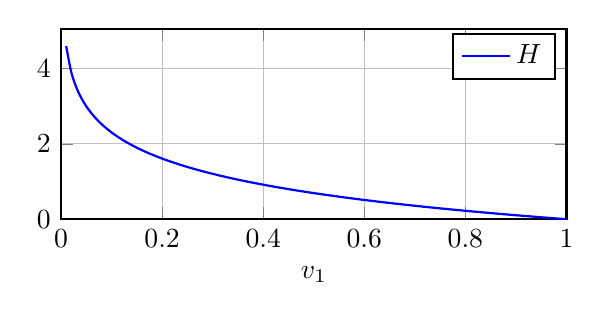
\begin{tikzpicture}
  \begin{axis}[domain=0:1, samples=100, smooth, no markers, grid, ymin=0, xmin=0, xmax=1, width=8cm, height=4cm, thick, xlabel=$v_1$]
    \addplot { -(1*ln(x) + 0 * ln(1 - x)) };
    \legend{$H$};
  \end{axis}
\end{tikzpicture}
\end{center}

\end{frame}


\begin{frame}
  \frametitle{Loss Functions}
  \framesubtitle{Cross-Entropy}

Note that $H$ can reach $0$ only if any $u_t=1$
\begin{itemize}
    \item In general $H(\vu,\vv)=H(\vu)$ if $\vu=\vv$ %
\end{itemize}

\medskip

\begin{center}
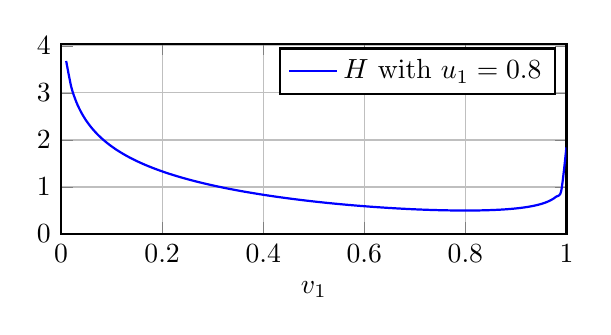
\begin{tikzpicture}
  \begin{axis}[domain=0:1, samples=100, smooth, no markers, grid, ymin=0, xmin=0, xmax=1, width=8cm, height=4cm, thick, xlabel=$v_1$]
    \addplot { -(0.8*ln(x) + 0.2 * ln(1 - x)) };
    \legend{$H$ with $u_1=0.8$}; %
  \end{axis}
\end{tikzpicture}
\end{center}

\end{frame}


\begin{frame}
  \frametitle{Loss Functions}
  \framesubtitle{Cross-Entropy Loss}

To utilize the cross-entropy for classifier training we
\begin{itemize}
    \item Let $\vu$ be our one-hot encoded class labels
    \item Let $\vv$ be the predicted softmax class scores
\end{itemize}

\bigskip

$H$ measures how dissimilar true and predicted probabilities are
\begin{itemize}
    \item How well the classifier performs on a single sample
\end{itemize}

\bigskip

Note that $H(\vu,\vv)$ depends only on $u_t$ and $v_t$
\begin{itemize}
    \item $u_t=1$ so all other $u_k$ are $0$
\end{itemize}

\end{frame}


\begin{frame}
  \frametitle{Loss Functions}
  \framesubtitle{Cross-Entropy Loss}

On this basis we calculate the \emph{cross-entropy loss} on $\cD$ as
\[
    L(\bth)=\frac{1}{S} \sum_{s=1}^S H(\vo^s,\text{softmax}(f(\vx^s;\bth)))
\]

\bigskip

Average cross-entropy over some dataset $\cD$
\begin{itemize}
    \item How good our classifier performs on $\cD$ on average
\end{itemize}

\end{frame}


\begin{frame}
  \frametitle{Gradient Descent}
  \framesubtitle{Motivation}

We now know how to compute $L(\bth)$ for classification

\bigskip

Need a way to minimize $L(\bth)$
\begin{itemize}
    \item Maximizes the training set classification performance %
    \item And hopefully also validation/test performance (more later) %
\end{itemize} 

\bigskip
 
$L(\bth)$ is not linear in $\bth$ %
\begin{itemize}
    \item Need a \emph{nonlinear optimization} algorithm
    \item \emph{Gradient descent} is popular choice in deep learning
\end{itemize}

\end{frame}


\begin{frame}
  \frametitle{Gradient Descent}
  \framesubtitle{Introduction}

Assume terrain corresponds to $L(\bth)$ with $\dim(\bth)=2$

\bigskip

\begin{center}
\includegraphics[width=7cm]{images/mp.jpg}
\end{center}

\end{frame}


\begin{frame}
  \frametitle{Gradient Descent}
  \framesubtitle{Introduction}

How do I get from location $\bth$ to location of minimum $\hat{\bth}$?

\bigskip

\begin{center}
\begin{tikzpicture}
    \node[anchor=south west,inner sep=0] (image) at (0,0) {\includegraphics[width=7cm]{images/mp.jpg}};
    \node[tuwcvl_inf_red,scale=1.5] at (4,2) {$\bth$};
    \node[tuwcvl_inf_red,scale=1.5] at (6.6,3.5) {$\hat{\bth}$};
    \draw[tuwcvl_inf_red,thick,dashed] (4,2) -- (5.7,1.1);
    \draw[tuwcvl_inf_red,thick,dashed] (6.6,3.2) -- (6.6,1.2);
    \draw[tuwcvl_inf_red,thick,dashed,opacity=0.4] (6.6,1.2) -- (6.6,0.5);
\end{tikzpicture}
\end{center}

\end{frame}


\begin{frame}
  \frametitle{Gradient Descent}
  \framesubtitle{Introduction}

Without actually seeing $L(\bth)$?

\bigskip

\begin{center}
\begin{tikzpicture}
    \node[anchor=south west,inner sep=0] (image) at (0,0) {\includegraphics[width=7cm]{images/mp.jpg}};
    \node (image) at (5.8,3.1) {\includegraphics[width=1cm]{images/bag.png}};
    \node[tuwcvl_inf_red,scale=1.5] at (4,2) {$\bth$};
    \node[tuwcvl_inf_red,scale=1.5] at (6.6,3.5) {$\hat{\bth}$};
    \draw[tuwcvl_inf_red,thick,dashed] (4,2) -- (5.7,1.1);
    \draw[tuwcvl_inf_red,thick,dashed] (6.6,3.2) -- (6.6,1.2);
    \draw[tuwcvl_inf_red,thick,dashed,opacity=0.4] (6.6,1.2) -- (6.6,0.5);
\end{tikzpicture}
\end{center}

\end{frame}


\begin{frame}
  \frametitle{Gradient Descent}
  \framesubtitle{Introduction}

Feel slope with feet, step in direction that feels steepest
\begin{itemize}
    \item Again and again until ground feels flat
\end{itemize}

\medskip

\begin{center}
\begin{tikzpicture}
    \node[anchor=south west,inner sep=0] (image) at (0,0) {\includegraphics[width=7cm]{images/mp.jpg}};
    \node (image) at (5.8,3.1) {\includegraphics[width=1cm]{images/bag.png}};
    \node[tuwcvl_inf_red,scale=1.5] at (4,2) {$\bth$};
    \node[tuwcvl_inf_red,scale=1.5] at (6.6,3.5) {$\hat{\bth}$};
    \draw[tuwcvl_inf_red,thick,dashed] (4,2) -- (5.7,1.1);
    \draw[tuwcvl_inf_red,thick,dashed] (6.6,3.2) -- (6.6,1.2);
    \draw[tuwcvl_inf_red,thick,dashed,opacity=0.4] (6.6,1.2) -- (6.6,0.5);
\end{tikzpicture}
\end{center}

\end{frame}


\begin{frame}
  \frametitle{Gradient Descent}
  \framesubtitle{Definition}

\emph{Iterative Optimization} algorithm

\bigskip

In every iteration we
\begin{itemize}
    \item Compute gradient $\bth'=\nabla L(\bth)$
    \item Update parameters $\bth = \bth - \alpha\bth'$
\end{itemize}

\bigskip

Hyperparameter $\alpha>0$ is called \emph{learning rate}
\begin{itemize}
    \item Final \emph{step size} is $\alpha\,\lVert\bth'\rVert$ %
\end{itemize}

\end{frame}


\begin{frame}
  \frametitle{Gradient Descent}
  \framesubtitle{Gradients}

Let $f(x_1,\dots,x_n)$ be a differentiable, real-valued function

\bigskip

The \emph{partial derivative} $f_{x_i}$ of $f$ with respect to $x_i$
\begin{itemize}
    \item Is also a real-valued function $f_{x_i}(x_1,\dots,x_n)$
\end{itemize}

\bigskip

$f_{x_i}(\vx)$ encodes
\begin{itemize}
    \item How fast $f$ changes with argument $x_i$
    \item At some location $\vx$
\end{itemize}

\end{frame}


\begin{frame}
  \frametitle{Gradient Descent}
  \framesubtitle{Gradients}

\emph{Gradient} $\nabla f$ is vector of all partial derivatives of $f$
\begin{itemize}
    \item $\nabla f=\left(f_{x_1},\dots,f_{x_n}\right)$
    \item Vector-valued function $\RR^n\mapsto\RR^n$
\end{itemize}

\bigskip

$\nabla f(\vx)=(f_{x_1}(\vx),\dots,f_{x_n}(\vx))$ encodes
\begin{itemize}
    \item How fast $f$ changes with all arguments $x_1\cdots x_n$
    \item At some location $\vx$
\end{itemize}

\end{frame}


\begin{frame}[fragile]
  \frametitle{Gradient Descent}
  \framesubtitle{Gradients}

\begin{center}
    \copyrightbox[b]
    {
    \begin{tikzpicture}
        \node[anchor=south west,inner sep=0] (image) at (0,0) {\includegraphics[width=7.5cm]{images/gradient-2d.pdf}};
        \node at (1.7, 0.6) {$x_1$};
        \node at (6.3, 0.6) {$x_2$};
        \node at (-0.1,2.9) {$f(\vx)$};
        \node at (-0.1,1.2) {$\nabla f(\vx)$};
        \draw[tuwcvl_inf_red,thick] (0.45,1.22) -- (2.6,2);
    \end{tikzpicture}
    }
    {\centering Image adapted from wikimedia.org}
\end{center}

\end{frame}


\begin{frame}
  \frametitle{Gradient Descent}
  \framesubtitle{Gradients}

$\nabla f(\vx)$ specifies how $f$ changes locally at $\vx$
\begin{itemize}
    \item Points in direction of greatest increase
    \item Norm equals magnitude of increase
\end{itemize}

\bigskip

Exactly what we need to minimize $L$
\begin{itemize}
    \item Compute direction of greatest increase $\nabla L(\bth)$
    \item Move in the opposite direction
\end{itemize}

\end{frame}


\begin{frame}
  \frametitle{Gradient Descent}
  \framesubtitle{Remarks}

Must stop if $\nabla L(\bth)\approx\vec{0}$ (if norm is close to $0$) %
\begin{itemize}
    \item No information where to go next
    \item $L$ is flat at current location
    \item The case if we are at $\hat{\bth}$ (but not only then)
\end{itemize}

\end{frame}


\begin{frame}
  \frametitle{Gradient Descent}
  \framesubtitle{Remarks}

Simple and general algorithm
\begin{itemize}
    \item Requires only that $f$ is differentiable and real-valued
    \item Efficient (requires only first derivatives)
\end{itemize}

\bigskip

Several (possible) limitations
\begin{itemize}
    \item Performs poorly for many $f$
    \item But works remarkably well with deep learning models
\end{itemize}

\bigskip

In a later lecture we will cover
\begin{itemize}
    \item Various improvements to gradient descent training
    \item How to compute $\nabla L$ efficiently
\end{itemize}

\end{frame}


\begin{frame}
  \frametitle{Machine Learning for Image Classification}
  \framesubtitle{Demo}
  
  \begin{center}
      \copyrightbox[b]
      {\includegraphics[width=9cm]{images/linear-classifier-demo.jpg}}
      {\centering Image from \href{http://vision.stanford.edu/teaching/cs231n-demos/linear-classify/}{cs231n.github.io}}
  \end{center}
  
\end{frame}


\begin{frame}
  \frametitle{Machine Learning for Image Classification}
  \framesubtitle{Remarks}

We factorized machine learning into basic blocks
\begin{itemize}
    \item Output shape, model, loss function, optimizer
\end{itemize}

\bigskip

Flexible approach that (hopefully) makes things clearer
\begin{itemize}
    \item Different problem? Change output shape and loss function
    \item Want more capacity? Change the model
    \item Optimization not going well? Change optimizer
\end{itemize}

\end{frame}


\renewcommand\emph[1]{\oldemph{#1}}

\begin{frame}
\frametitle{Bibliography}

[1] Prince. Computer Vision Models. 2012.

\end{frame}


\end{document}
